\chapter{实验}
\label{cha:exp}
本章介绍验证模型结构所进行的实验。首先,使用Transformer作为基线模型实验了单任务学习下的模型性能,接着使用相同的超参设定实验了~\ref{sec:mtl_tf}~节介绍的四种多任务Transformer的性能。具体地,在第~\ref{sec:task}~节介绍实验任务,在第~\ref{sec:ds}~节介绍数据集相关信息,在第~\ref{sec:results}~节介绍实验结果。最后,~\ref{sec:analysis}~节给出了实验分析。

\section{任务描述}
\label{sec:task}
我们在\emph{文本分类}(Text Classification)这一经典NLP任务上进行实验。事实上,很多NLP问题都可以归为文本分类的范畴,例如情感分析(Sentiment Analysis, SA)、自然语言推理(Natural Language Inference, NLI)等。在目前被广泛使用的多任务基准数据集GLUE\cite{DBLP:conf/emnlp/WangSMHLB18}中,所有任务都可以被归为文本分类任务。

文本分类即将一段文本归到某个特定的预先定义的类别。待分类的文本通常是一个句子(如情感分析)或一个句子对(如自然语言推理)。需要注意的是,这里的一个句子并不一定是常规意义上以一个句号为结束标识符的一句话,也有可能包含多句话。文本分类任务在现实生活中有着广泛的应用,如自动分析产品评价、微博情感分析、文档归类等等。文本分类任务需要模型能够抽取出易于分类的句子表示,即需要句子级的文本表示模型。

具体地,本文在\emph{情感分析}任务上进行实验:对于一段用户生成的文本,模型需要判断其情感极性为正向还是负向。然而对于不同领域的文本通常需要关注不同的特征,例如在食物类的评论文本中模型应当更加关注“好吃”、“美味”等词,而在电影评论文本中应当更加关注“好看”、“烂片”等词语。同时,不同领域的文本分类任务常常也需要某些通用的特征,如“很棒”、“失望”等词在所有与情感倾向有关的分类任务中都是应当被关注的。而事实上,在某个特定的领域内,文本数据量常常是有限的,这种情况下单任务学习通常难以取得很好的效果,可以通过多任务学习来利用其他领域的相关知识帮助分类。

\section{数据集}
\label{sec:ds}
我们的基线单任务模型以及多任务模型在16个文本分类数据集上进行了对比实验,其中的前14个数据集来自亚马逊的产品评论\footnote{\url{https://www.cs.jhu.edu/˜mdredze/datasets/ sentiment/}},但是来自各自不同的领域,如图书、电子、光盘等。该部分数据由Blitzer等人\cite{DBLP:conf/acl/BlitzerDP07}收集而成,其余两个数据集IMDB\cite{DBLP:conf/acl/MaasDPHNP11}和MR\cite{DBLP:conf/acl/PangL05}则来自电影评论。每个数据集包含约2000个样本,其中70\%划分为训练集,10\%划分为验证集,20\%划分为测试集。数据集的具体统计信息见表~\ref{tb:dataset}。

\begin{table}[htb]
	\centering
	\caption{数据集统计数据}
	\begin{tabular}{ccccccc}
		\toprule[2pt]
		数据集&训练集大小&验证集大小&测试集大小&类别数&平均长度&词表大小\\
		\midrule[1pt]
		Books& 1400& 200& 400& 2& 159& 19K\\
		Elec& 1398& 200& 400& 2& 101& 11K\\
		DVD& 1400& 200& 400& 2& 173& 20K\\
		Kitchen& 1400& 200& 400& 2& 89& 9K\\
		Apparel& 1400& 200& 400& 2& 57& 7K\\
		Camera& 1397& 200& 400& 2& 130& 9K\\
		Health& 1400& 200& 400& 2& 81& 9K\\
		Music& 1400& 200& 400& 2& 136& 17K\\
		Toys& 1400& 200& 400& 2& 90& 10K\\
		Video& 1400& 200& 400& 2& 156& 17K\\
		Baby& 1300& 200& 400& 2& 104& 8K\\
		Mag& 1370& 200& 400& 2& 117& 11K\\
		Soft& 1315& 200& 400& 2& 129& 11K\\
		Sports& 1400& 200& 400& 2& 94& 10K\\
		IMDB& 1400& 200& 400& 2& 269& 25K\\
		MR& 1400& 200& 400& 2& 21& 7K\\
		\bottomrule[2pt]
	\end{tabular}
	\label{tb:dataset}
\end{table}

这里所有数据集中的样本都被标注为两个类别,分别表示情感极性的正向和负向。如表~\ref{tb:dataset}~所示,虽然各数据集均属于情感分析任务,且数据规模相当,但其样本来自不同的产品领域,平均句子长度和词汇量大小也各不相同,各个任务的难度也有所差别。

表~\ref{tb:examples}~给出了其中几个数据集中的部分样例。
\begin{table}[htb]
\centering
\caption{数据集中的部分样本}
\begin{tabular}{m{1.5cm}m{10cm}m{2cm}}
\toprule[2pt]
领域 & 样例 & \ 类别\\
\midrule[1pt]
Books&It is a very dry book and hard to stay interested in. I am barely able to stay awake while reading it. It does have some interesting things.& \ Negative\\
Mag&The magazine was shipped in a timely manner, i would use this vendor again.& \ Positive\\
Elec&Very pleased with the high capacity cartridge with my epson stylus cx6600.& \ Positive\\
MR&Just a big mess of a movie, full of images and events, but no tension or surprise.& \ Negative\\
Health&Its quality is cheap and poorly made. I bought two thinking it was a good deal but I threw them out after 2 days because the on/off switch didn't work.& \ Negative\\
\bottomrule[2pt]
\end{tabular}
\label{tb:examples}
\end{table}

\section{实验结果}
\label{sec:results}
使用训练集对单任务基线模型以及四种多任务Transformer模型进行训练,选择在验证集上表现最好的模型进行测试。测试集上各模型的分类准确率如表~\ref{tb:results}~所示。可见,本文的四个多任务模型在十六个文本分类任务上均超过了单任务训练的表现,验证了多任务学习在Transformer模型上的有效性。其中,L-I结构在四种多任务架构中表现最好,S-P结构表现最差。注意到两种逐层共享的结构:L-I结构和L-E结构,取得了相对传统硬共享结构(S-P结构和S-C结构)更高的分类准确率,这说明在每一层都形成任务特定表示的模式相比在网络的顶层获取特征更为合理。随着任务之间差异性的增大,我们有理由认为L-I结构和L-E结构的共享模式将表现出更大的优越性。

\begin{table}[htb]
	\centering
	\caption{模型在测试集上的分类准确率}
	\begin{tabular}{c|cccccc}
		\toprule[2pt]
		\multirow{2}*{数据集}&\multirow{2}*{单任务}&\multicolumn{4}{c}{多任务}\\
		\cline{3-6}
		&&S-P结构& S-C结构& L-I结构& L-E结构\\
		\midrule[1pt]
		Books& 83.50& 82.50& 84.00& 85.00& 84.50\\
		Elec& 79.50& 82.50& 83.50& 84.75& 85.75\\
		DVD& 82.75& 84.50& 85.50& 85.75& 85.75\\
		Kitchen& 79.50& 83.50& 85.00& 89.00& 87.75\\
		Apparel& 82.75& 85.50& 86.75& 86.00& 85.75\\
		Camera& 81.75& 84.25& 85.00& 87.00& 89.00\\
		Health& 86.00 & 85.50& 87.50& 88.00& 86.75\\
		Music& 76.50& 83.00& 83.00& 82.75& 81.50\\
		Toys& 80.00& 84.75& 86.25& 88.25& 86.50\\
		Video& 84.75& 81.25& 85.50& 86.50& 84.25\\
		Baby& 81.00 &87.75& 85.50& 87.25& 87.50\\
		Mag& 89.00& 85.00& 91.00& 89.75& 89.25\\
		Soft& 86.50& 86.00& 88.75& 86.50& 87.75\\
		Sports& 80.25& 84.25& 83.75& 86.00& 85.50\\
		IMDB& 80.75& 84.75& 85.00& 84.50& 84.50\\
		MR& 75.25& 76.00& 75.75& 78.00& 76.50\\
		\rowcolor{lightgray}
		AVG.& 81.86& 83.81& 85.11& \textbf{85.94}& 85.53\\
		\bottomrule[2pt]
	\end{tabular}
	\label{tb:results}
\end{table}

值得注意的是,本文的四种多任务Transformer结构相比单任务学习下的设定并不会增加过多的参数,这一特点与硬共享模式类似,相对的,传统的软共享模式常常需要很多额外的参数。表~\ref{tb:params}~给出了单任务Transformer以及四种多任务Transformer结构的参数量,各模型的网络层数均为四层,参数量的统计忽略了词嵌入、位置编码等模型无关的参数。

\begin{table}[htb]
	\centering
	\caption{各模型参数量对比}
	\begin{tabular}{cccc}
		\toprule[2pt]
		类型&模型&参数量&相对增量\\
		\midrule[1pt]
		单任务&Transformer&$2,773,150$‬&-\\
		\multirow{4}*{多任务}&S-P结构&$2,782,180$&$+0.32\%$\\
		&S-C结构&$2,782,480$&$+0.34\%$\\
		&L-I结构&$2,786,980$&$+0.50\%$\\
		&L-E结构&$2,786,980$&$+0.50\%$\\
		\bottomrule[2pt]
	\end{tabular}
	\label{tb:params}
\end{table}

可见,本文提出的几种多任务Transformer结构相比单任务模型并不会增加过多的参数,即使在十六个任务的情形下,L-I结构也仅增加了0.5\%的参数量,但能够降低22.5\%的错误率。

另外,在实践中,神经网络的层数通常是一个比较重要的超参数,模型性能有时会由于层数的不同而产生较大差异。之前的实验中使用的模型均为4层Transformer,为探究多任务Transformer结构对网络层数的敏感性,我们实验了四种结构在不同层数下的平均分类准确率,结果如图~\ref{fig:layer_dis}~所示。

在各个层数设定中,逐层共享结构(L-I结构和L-E结构)均优于传统的硬共享结构(S-P结构和S-C结构),且L-I结构在三种设定中都取得了最优准确率,这一实验结果证明了模型的鲁棒性,也表明了表~\ref{tb:results}~数据的可信性。另外,在二、四、六层三种设定中,模型被设定为四层在除S-P结构中都在测试集上表现出了最高分类准确率,而S-P结构则随着层数增长而准确率下降,没有获得模型复杂度增长带来的收益。

\begin{figure}[h!]
	\centering
	\begin{tikzpicture}
	\begin{axis}[
	xlabel={层数},
	ylabel={准确率},
	legend style={
		cells={anchor=east},
		legend pos=outer north east,
	}
	]
	
	\addplot coordinates{
		(2, 0.8547)
		(4, 0.8594)
		(6, 0.8523)
	};
	
	\addplot coordinates{
		(2, 0.8539)
		(4, 0.8553)
		(6, 0.8500)
	};
	
	\addplot [mark=x]coordinates {
		(2, 0.8451)
		(4, 0.8381)
		(6, 0.8167)
	};
	
	\addplot coordinates{
		(2, 0.8484)
		(4, 0.8511)
		(6, 0.8478)
	};
	\legend{L-I结构,L-E结构,S-P结构,S-C结构}
	\end{axis}
	\end{tikzpicture}
	\caption{网络层数对测试集准确率的影响}
	\label{fig:layer_dis}
\end{figure}
\section{实验分析}
\label{sec:analysis}
Transformer模型由于基于注意力机制,可以将注意力分数矩阵进行可视化来揭示模型的机理,因而相比其他深度模型具备较好的可解释性。另外,在多任务学习中,相关任务之间的交互关系一直是很多研究人员关注的重点问题。

考虑到以上两点,本节根据两个来自不同领域的示例输入对L-E结构中最后一层的注意力进行可视化分析,以探究模型有效的原因以及任务之间的关系。注意力矩阵的可视化结果如图~\ref{fig:l-e-attn}~所示,每一行代表一个注意力头,每一列代表输入中的一个位置,其中前16个位置为任务标识符,后续位置为句子中的各个单词,两段输入文本分别来自杂志(Mag)数据集和电影评论(MR)数据集。

\begin{figure}[htb]
\centering

\subfloat[杂志(Mag)]{
	\centering
	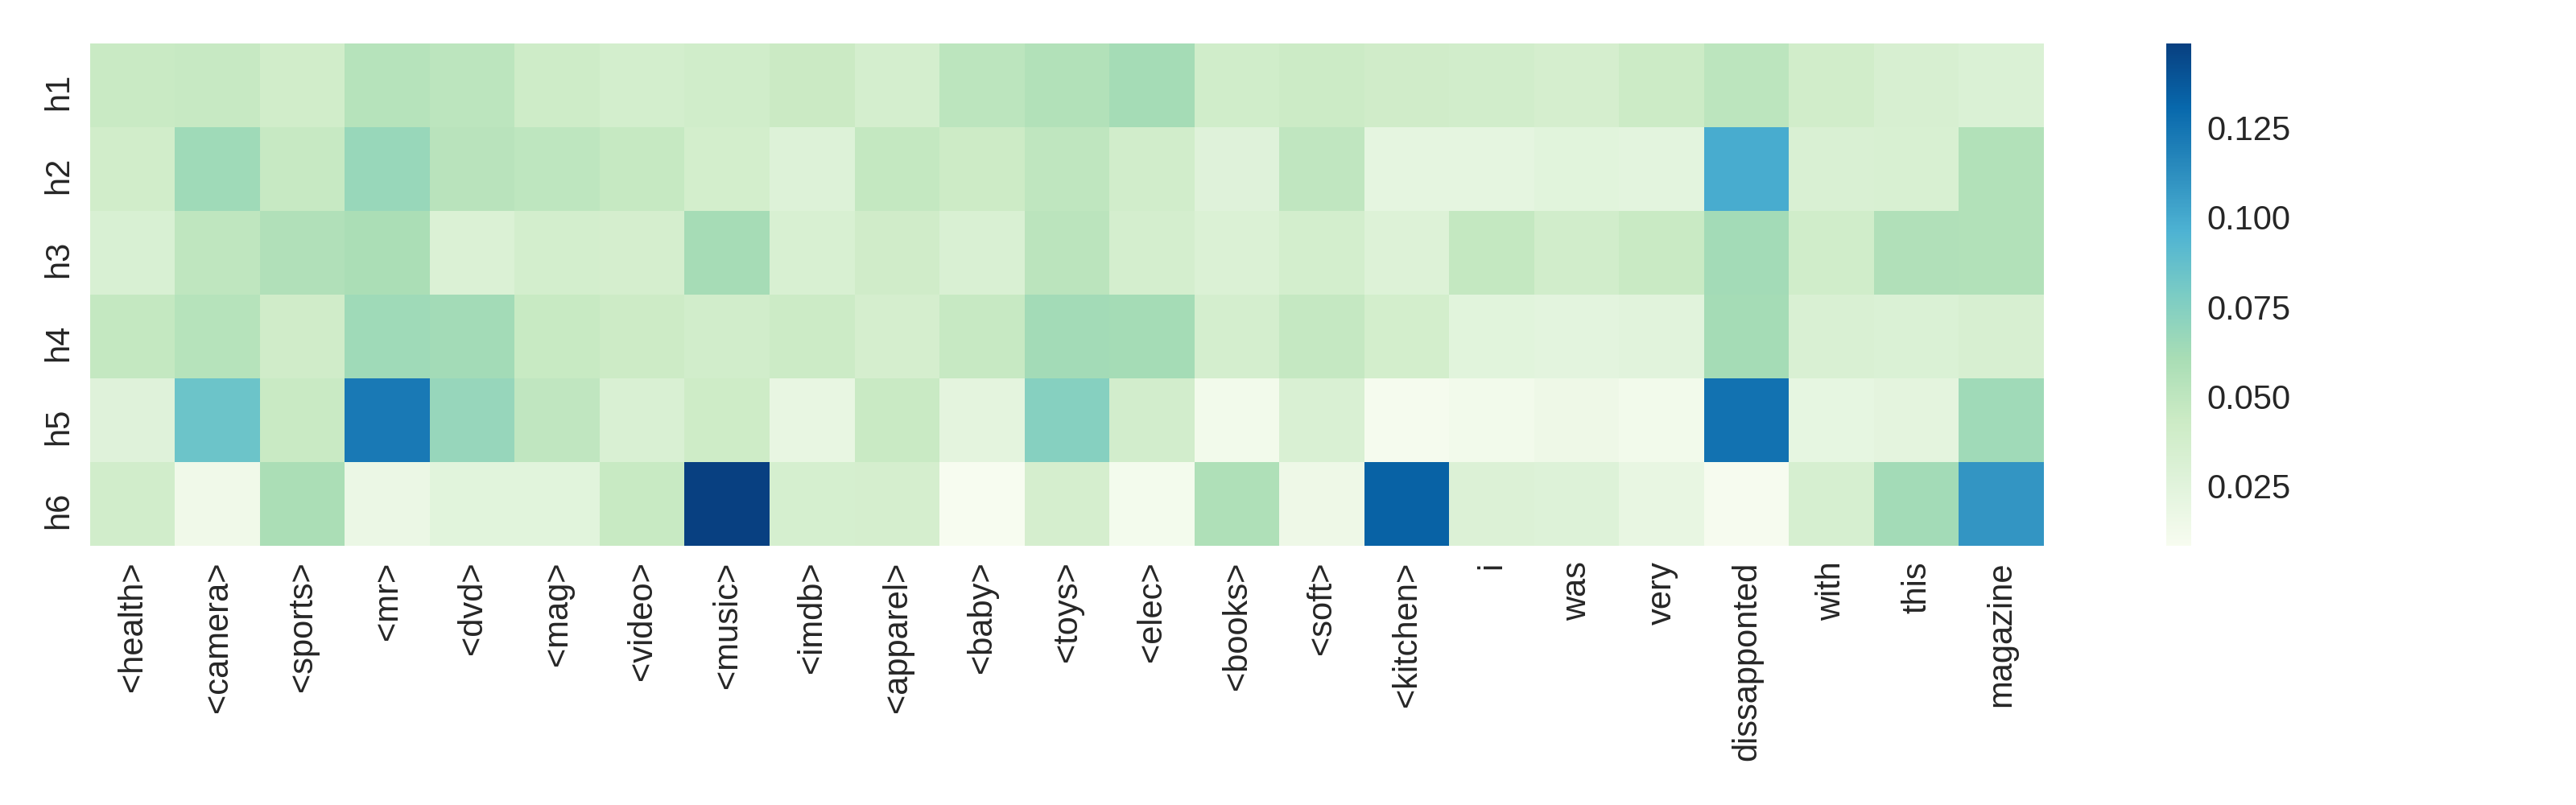
\includegraphics[scale=0.4]{viz-mag.png}
}

\subfloat[电影评论(MR)]{
	\centering
	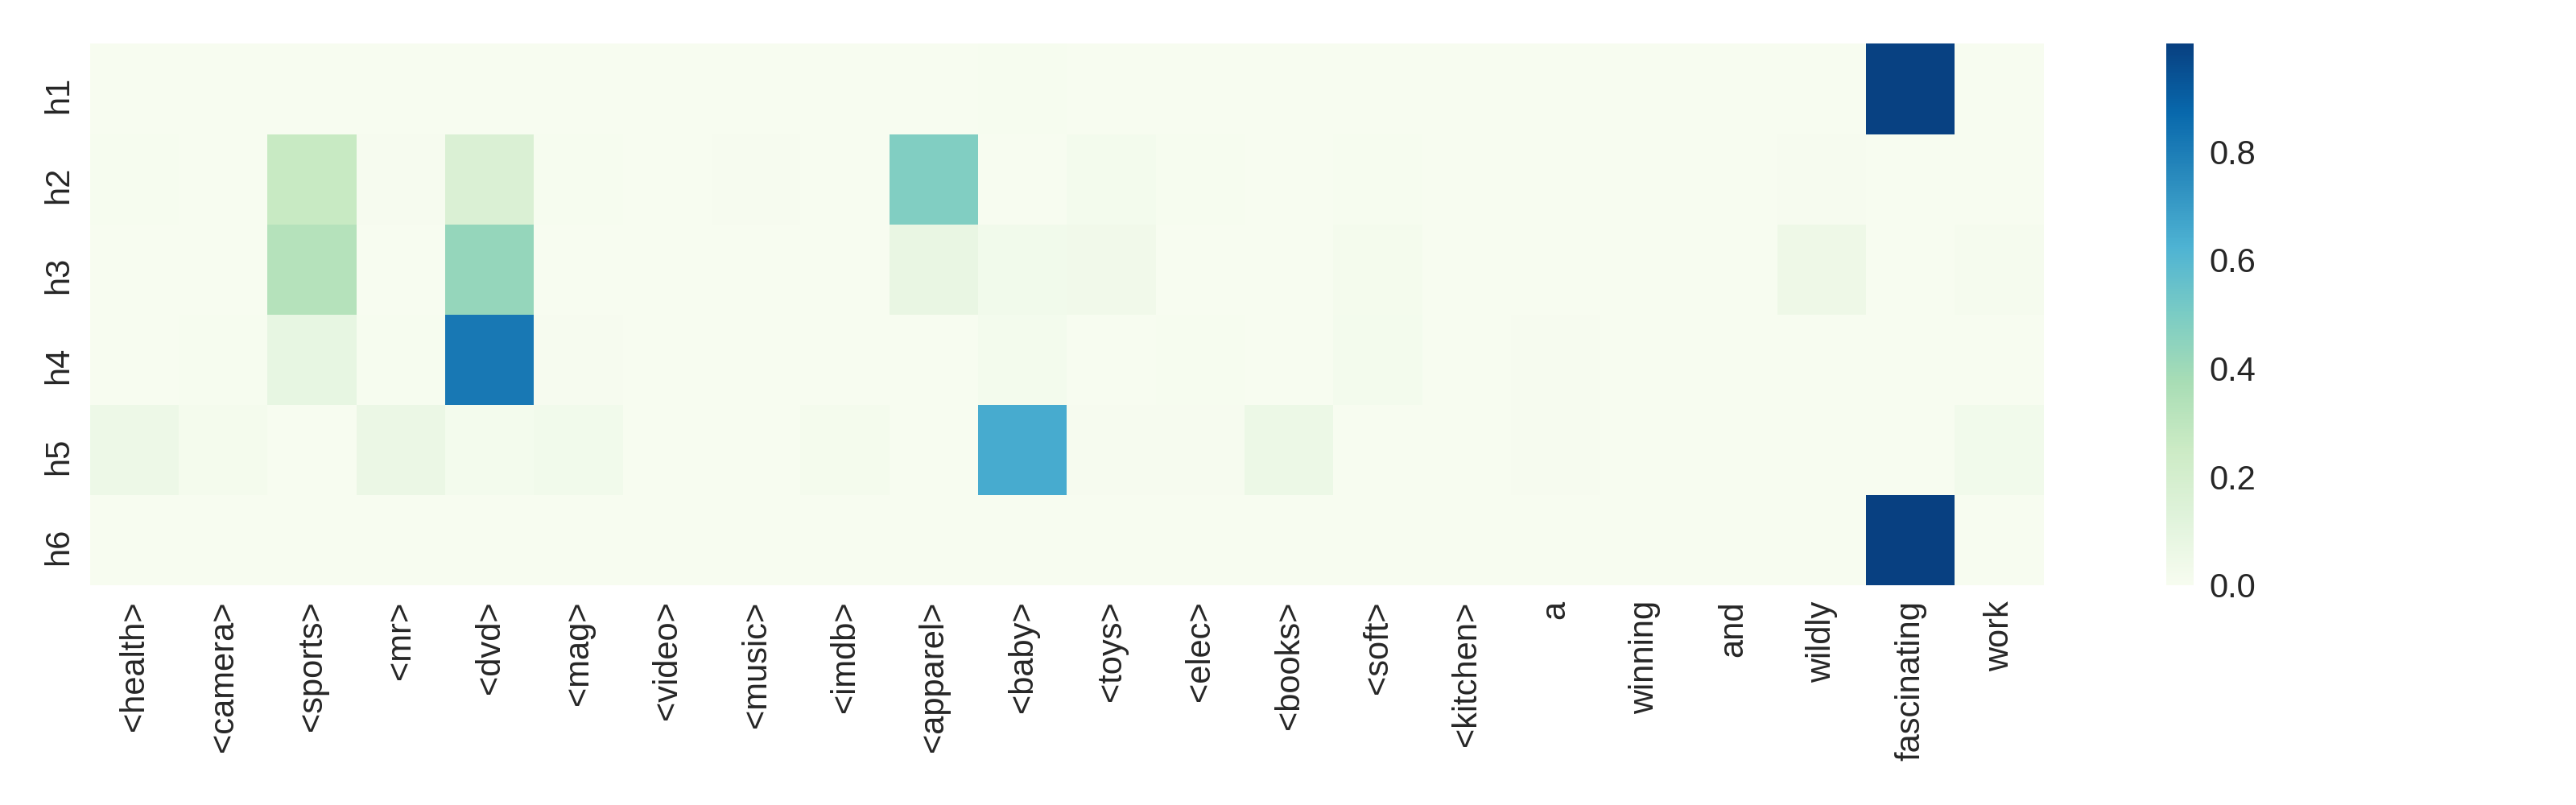
\includegraphics[scale=0.4]{viz-mr.png}
}
\caption{L-E结构注意力可视化}
\label{fig:l-e-attn}
\end{figure}

可见,杂志领域情感分析任务与音乐和厨具领域的情感分析任务有很强的相关性,而电影评论情感分析任务与影碟产品领域的任务最为相似。同时还可以注意到,L-E模型还注意到了输入句子中具有较强情感指示性的单词,如图~\ref{fig:l-e-attn}~(a)中的disappointed(失望的)以及图~\ref{fig:l-e-attn}~(b)中的fascinating(惊艳的),这为模型的预测提供了一定的可解释性。